\section{ Melhoria de processo (TO - BE)}

Essa seção vem  propor a solução de redesign  dos processos
anteriormente apresentados, com o objetivo de resolver os convenientes
já listados, tendo como base os conhecimentos e informações coletadas
durante a execução do projeto. Levando em consideração essa adaptação o
local e os fatores da empresa.

Para a Gestão do Conhecimento e Auto-ajuda, uma da=os principais pontos da
análise foi a ausência de gestão do conhecimento.

Por exemplo, isso ter o uso da gestão fo conhecimento pode diminuir dependência de
pessoal qualificado que limita as oportunidades de auto-ajuda.
Portanto, é proposto a implementação de  uma base de conhecimento adequada
para uso interno e aberto dos usuários. Para prover essa gestão de conhecimento
e auto ajuda será preciso incluir outros pontos que são listados a seguir.
A base de conhecimento será lançada como uma extensão do suporte web page


\begin{itemize}[noitemsep]

		\item Manual para suporte dos usuários
		\item Documentação completa dos produtos de software
		\item Documentação de Problemas comuns
		\item Base de dados de erros e suas soluções alternativas
		\item Base de dados de improvement sugestions
		\item Monitoramento de performace \\

\end{itemize}

 \textbf{Monitoramento de performace:}
Para obter os indicadores chave de desempenho, foi criado uma
matrix de fatores de críticos de sucesso sugeridos.
Isso possibilitou criar relações e definir quais indicadores
correspondem as necessidades esperadas, observados na tabela 1 abaixo.
	A ferramenta usada para a gerência deve gerar dois tipos de relatório, online
	e offline. A ferramenta deve informar os relatórios online diariamente, já
	para os relatórios offline deve ser gerados em um período de tempo de 30 dias.
	O monitoramento deve trazer também o índice de satisfação do cliente,
	gerando um fluxo da seguinte maneira, após a finalização de um atendimento
	será solicitado que o usuário participe da pesquisa de satisfação, como
	primeira ação foi necessário achar os indicadores chave de performace,
	onde foi possivel mapear o relacionamento desses indicadores chave com os fatores
	critícos de sucesso

  \clearpage% Flush earlier floats (otherwise order might not be correct)
  \thispagestyle{empty}% empty page style (?)
  \begin{landscape}% Landscape page
			% Please add the following required packages to your document preamble:
% \usepackage{multirow}
% \usepackage[table,xcdraw]{xcolor}
% If you use beamer only pass "xcolor=table" option, i.e. \documentclass[xcolor=table]{beamer}
\begin{table}[]
\centering
\caption{Lista de indicadores de performace}
\label{my-label}
\begin{tabular}{|c|l|c|c|c|c|}
\hline
\multicolumn{2}{|c|}{}                                                                                                                                                  & \multicolumn{4}{c|}{\cellcolor[HTML]{67FD9A}\textbf{Fatores de sucesso}}                                                                                                                                                                                                                                                                                                                                                                                                                           \\ \cline{3-6}
\multicolumn{2}{|c|}{\multirow{-2}{*}{}}                                                                                                                                & \cellcolor[HTML]{9AFF99}                                                                                              & \cellcolor[HTML]{9AFF99}                                                                                                   & \cellcolor[HTML]{9AFF99}                                                                                                  & \cellcolor[HTML]{9AFF99}                                                                                          \\ \cline{1-2}
\multicolumn{2}{|c|}{\cellcolor[HTML]{FFFC9E}\textbf{Indicadores de performace}}                                                                                        & \multirow{-2}{*}{\cellcolor[HTML]{9AFF99}\textbf{\begin{tabular}[c]{@{}c@{}}Menor tempo \\ de resposta\end{tabular}}} & \multirow{-2}{*}{\cellcolor[HTML]{9AFF99}\textbf{\begin{tabular}[c]{@{}c@{}}Menor tempo \\ de processamento\end{tabular}}} & \multirow{-2}{*}{\cellcolor[HTML]{9AFF99}\textbf{\begin{tabular}[c]{@{}c@{}}Volume menor \\ de requisições\end{tabular}}} & \multirow{-2}{*}{\cellcolor[HTML]{9AFF99}\textbf{\begin{tabular}[c]{@{}c@{}}Menos tarefa \\ humana\end{tabular}}} \\ \hline
\multicolumn{2}{|c|}{\cellcolor[HTML]{FFFFC7}\begin{tabular}[c]{@{}c@{}}Tempo médio de resposta \\ do primeiro contato\end{tabular}}                                    & secundária                                                                                                            & secundária                                                                                                                 &                                                                                                                           &                                                                                                                   \\ \hline
\multicolumn{2}{|c|}{\cellcolor[HTML]{FFFFC7}\begin{tabular}[c]{@{}c@{}}Número de solicitações com \\ tempo de resposta violado\end{tabular}}                           & primária                                                                                                              & secundária                                                                                                                 &                                                                                                                           &                                                                                                                   \\ \hline
\multicolumn{2}{|c|}{\cellcolor[HTML]{FFFFC7}Tempo médio de resposta}                                                                                                   & secundária                                                                                                            & secundária                                                                                                                 &                                                                                                                           &                                                                                                                   \\ \hline
\multicolumn{2}{|c|}{\cellcolor[HTML]{FFFFC7}\begin{tabular}[c]{@{}c@{}}Número de solicitações \\ com tempo \\ de intervalo de \\ informação insuficiente\end{tabular}} & primária                                                                                                              & secundária                                                                                                                 &                                                                                                                           &                                                                                                                   \\ \hline
\multicolumn{2}{|c|}{\cellcolor[HTML]{FFFFC7}\begin{tabular}[c]{@{}c@{}}Tempo médio de \\ processamento\end{tabular}}                                                   &                                                                                                                       & primária                                                                                                                   & secundária                                                                                                                & secundária                                                                                                        \\ \hline
\multicolumn{2}{|c|}{\cellcolor[HTML]{FFFFC7}Custo médio por pedido}                                                                                                    &                                                                                                                       &                                                                                                                            &                                                                                                                           & primária                                                                                                          \\ \hline
\multicolumn{2}{|c|}{\cellcolor[HTML]{FFFFC7}Número de solicitações reabertas}                                                                                          &                                                                                                                       &                                                                                                                            & primária                                                                                                                  & secundária                                                                                                        \\ \hline
\multicolumn{2}{|c|}{\cellcolor[HTML]{FFFFC7}Índice de satisfação do cliente}                                                                                           & secundária                                                                                                            & secundária                                                                                                                 &                                                                                                                           &                                                                                                                   \\ \hline
\end{tabular}
\end{table}

    \end{landscape}
    \clearpage% Flush page

\subsection{Propostas de modelagem}
\subsubsection{Atendimento de requisição }
\begin{figure}[!h]
\caption{Gerencia de requisição - TO-BE}
\centering % para centralizarmos a figura
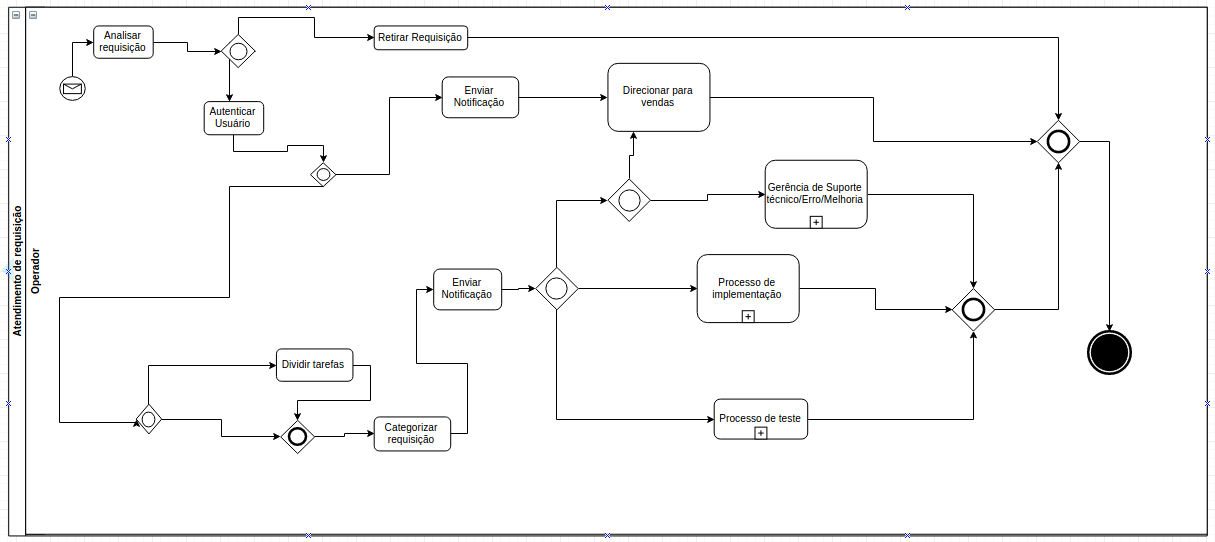
\includegraphics[width=15cm]{to_be/01_atendimento_de_requisicao.png}
\label{figura:atendimento_requisicao_to_be}
\end{figure}

\begin{itemize}[noitemsep]
	\item Analisar requisição
		\begin{itemize}
			\item Ler e entender a requisição
		\end{itemize}
	\item Autenticar Cliente
		\begin{itemize}
			\item Confirmar o registro do cliente no banco de dados
		\end{itemize}
	\item Dividir tarefas
		\begin{itemize}
			\item Dividir a requisição para diminuir a complexidade
		\end{itemize}
	\item Enviar Notificação
		\begin{itemize}
			\item Notificar o cliente sobre o progresso
		\end{itemize}
	\item Direcionar para vendas
		\begin{itemize}
			\item Direcionar o problema para o departamento de vendas
		\end{itemize}
	\item Categorizar requisição
		\begin{itemize}
			\item Categorizar a requisição
		\end{itemize}
	\item Retirar requisição
		\begin{itemize}
			\item Remover a requisição dos pedidos
		\end{itemize}
\end{itemize}

\subsubsection{Atendimento técnico}
\begin{figure}[!h]
\caption{Atendimento técnico - TO-BE}
\centering % para centralizarmos a figura
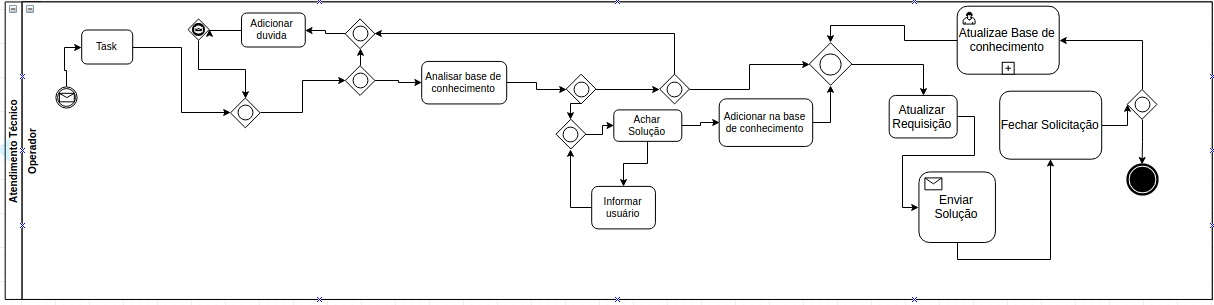
\includegraphics[width=15cm]{to_be/02_atendimento_tecnico.png}
\label{figura:suporte_tecnico_to_be}
\end{figure}

\begin{itemize}[noitemsep]
	\item Analisar requisição
	\begin{itemize}
		\item Ler e entender a requisição
	\end{itemize}
	\item Solicitar informações
		\begin{itemize}
			\item Solicita informações sobre a requisição para o cliente
		\end{itemize}
	\item Analisar Base de Conhecimento
		\begin{itemize}
			\item Procura pela solução na base de conhecimento
		\end{itemize}
	\item Achar Solução
		\begin{itemize}
			\item Acha uma nova solução para o problema
		\end{itemize}
	\item Adicionar na Base de Conhecimento
			\begin{itemize}
				\item Caso Adiciona uma nova solução na base de conhecimento
			\end{itemize}
	\item Atualizar Requisição
		\begin{itemize}
			\item Adiciona soluçao usada na requisição reportada
		\end{itemize}
	\item Enviar Solução
			\begin{itemize}
				\item Envia a solução do incidente
			\end{itemize}
	\item Fechar Requisição
			\begin{itemize}
				\item Fecha a requisição
			\end{itemize}
	\item Atualizar Base de Conhecimento
		\begin{itemize}
			\item Descreve a solução para adicionar na base de conhecimento
		\end{itemize}
	\item Informa o usuário
			\begin{itemize}
				\item Informar ao usuário o status da requisição
			\end{itemize}
\end{itemize}
\clearpage
\subsubsection{Atendimento para erro no sistema}

\begin{figure}[!h]
\caption{Atendimento para erro no sistema - TO-BE}
\centering % para centralizarmos a figura
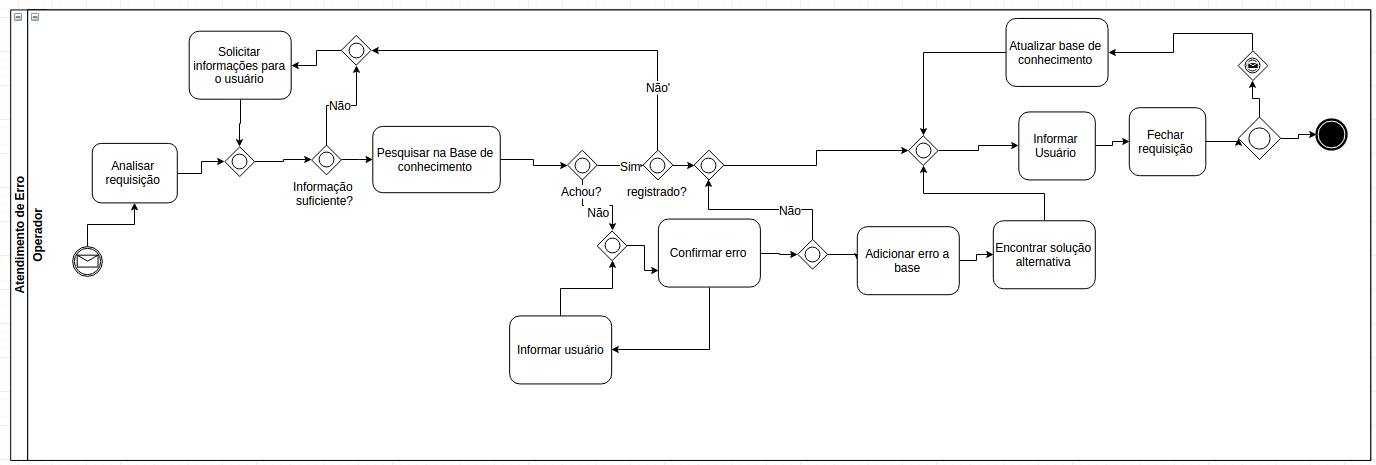
\includegraphics[width=15cm]{to_be/03_atendimento_de_erro.png}
\label{figura:atendimento_de_erro_to_be}
\end{figure}
\begin{itemize}[noitemsep]
	\item Analisar requisição
	\begin{itemize}
		\item Ler e entender a requisição
	\end{itemize}
	\item Solicitar informações para o usuário
	\begin{itemize}
		\item Solicita informações sobre a requisição para o cliente
	\end{itemize}
	\item Pesquisar na base de conhecimento
		\begin{itemize}
			\item Procurar por solução na base de conhecimento
		\end{itemize}
	\item Confimar Erro
		\begin{itemize}
			\item Confirmar se o erro não existe ainda na base de conhecimento
		\end{itemize}
	\item Adicionar erro Base de Conhecimento
		\begin{itemize}
			\item Adicionar a incidência do erro na base do conhecimento
		\end{itemize}
	\item Encontrar Solução alternativa
		\begin{itemize}
			\item É proposto uma solução para o erro
		\end{itemize}
	\item Fechar Requisição
		\begin{itemize}
			\item A requisição é finalizada
		\end{itemize}
	\item Atualizar Base de Conhecimento
	\begin{itemize}
		\item Descreve a solução para adicionar na base de conhecimento
	\end{itemize}
\end{itemize}


\subsubsection{Atendimento de Opinião/Melhoria}

\begin{figure}[!h]
\caption{Atendimento de Opinião/Melhoria - TO-BE}
\centering % para centralizarmos a figura
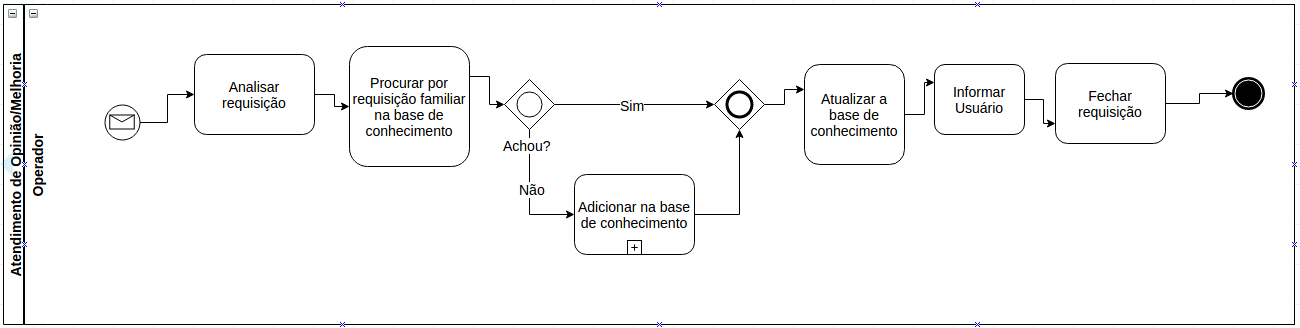
\includegraphics[width=15cm]{to_be/04_atendimento_de_melhoria.png}
\label{figura:atendimento_de_erro_to_be}
\end{figure}

\begin{itemize}[noitemsep]
	\item Analisar requisição
	\begin{itemize}
		\item Ler e entender a requisição
	\end{itemize}
	\item Procurar por requisição familiar na base de conhecimento
		\begin{itemize}
			\item Procurar na base familiaridades com outras requisições
		\end{itemize}
	\item Adicionar na Base de Conhecimento
		\begin{itemize}
			\item Adicionar na base de conhecimento
		\end{itemize}
	\item Atualizar base de conhecimento
	\begin{itemize}
		\item Descreve a melhoria para adicionar na base de conhecimento
	\end{itemize}
	\item Informar Usuário
	\begin{itemize}
		\item Informar ao usuário o status da requisição
	\end{itemize}
	\item Fechar requisição
	\begin{itemize}
		\item Fecha a requisição
	\end{itemize}
\end{itemize}



\subsection{Conclusão sobre o TO-BE}
Embora nem todas soluções projetadas se baseiem nos modelos propostos pelo ITIL
descritos no tópico 6 de Padrões e Normas, os principais e importantes conceitos
foram implementados.

Além disso, as soluções
baseiam-se não apenas no tópico 6 de Padrões e Normas, mas também de
circunstâncias reais, e cooperação com representantes da empresa.
Assim, a maior lição aprendida é que os processos predefinidos são
guias não dogmas.

Portanto, projetos padronizados precisam ser sempre
personalizados para atender às necessidades de uma empresa.
O desenvolvimento futuro é uma forma de desenvolvimento contínuo e
ajuste fino do processo. Dados de um uso de longo prazo serão necessários
para executar essa tarefa.
